\section{Results and analysis} \label{analysis}

For answering our research question, whether classical machine learning methods combined with suitable features can outperform neural network based approaches, the following results were achieved:
\begin{itemize}
	\item Investigation of feature importances (chapter \ref{ch:experimentDa})
	\item Hate speech statistics (chapter \ref{ch:experimentDb})
	\item Comparison of the classifier results (classical machine learning methods vs neural network based approaches) (chapter \ref{ch:experimentDc})
	\item Oversampled and undersampled datasets (chapter \ref{ch:experimentDd})
\end{itemize}

\subsection{Feature importances}
\label{ch:experimentDa}

\begin{table}[hbt!]
	\caption{Feature importance scores per classifier}
	\label{Tab:featureimportances}
	\begin{tabular}{|p{0.3\textwidth}|p{0.13\textwidth}|p{0.13\textwidth}|p{0.13\textwidth}|p{0.13\textwidth}|}
		\hline
		\textbf{feature}     & \textbf{Decision Tree} & \textbf{Random Forest} & \textbf{SVM} & \textbf{Logistic Regression} \\ \hline
		Unigrams      		 & \gradientOne{0.096833} & \gradientOne{0.110481} & \gradientTwo{0.116233} & \gradientTwo{0.340829} \\ \hline
		Bigrams       		 & \gradientOne{0.010989} & \gradientOne{0.030529} & \gradientTwo{0.163003} & \gradientTwo{0.288648} \\ \hline
		Trigrams       		 & \gradientOne{0.015111} & \gradientOne{0.041289} & \gradientTwo{1.389380} & \gradientTwo{2.009609} \\ \hline
		Hateful Words        & \gradientOne{0.165297} & \gradientOne{0.238533} & \gradientTwo{0.281878} & \gradientTwo{0.550001} \\ \hline
		Neutral Words        & \gradientOne{0.078015} & \gradientOne{0.060794} & \gradientTwo{0.092602} & \gradientTwo{0.211546} \\ \hline
		Exclamation Marks    & \gradientOne{0.015078} & \gradientOne{0.014925} & \gradientTwo{0.16408} & \gradientTwo{0.39866} \\ \hline
		Question Marks       & \gradientOne{0.015837} & \gradientOne{0.012568} & \gradientTwo{0.077828} & \gradientTwo{0.034885} \\ \hline
		Full Stop Marks      & \gradientOne{0.050472} & \gradientOne{0.039024} & \gradientTwo{0.015701} & \gradientTwo{0.018517} \\ \hline
		Interjections        & \gradientOne{0.001223} & \gradientOne{0.002545} & \gradientTwo{0.084760} & \gradientTwo{0.255209} \\ \hline
		All Caps Words       & \gradientOne{0.030842} & \gradientOne{0.025809} & \gradientTwo{0.036716} & \gradientTwo{0.119023} \\ \hline
		Quotation Marks      & \gradientOne{0.007124} & \gradientOne{0.011336} & \gradientTwo{0.083534} & \gradientTwo{0.197908} \\ \hline
		Words Total          & \gradientOne{0.176739} & \gradientOne{0.107484} & \gradientTwo{0.023188} & \gradientTwo{0.048423} \\ \hline
		Laughing Expressions & \gradientOne{0.002860} & \gradientOne{0.006506} & \gradientTwo{0.172888} & \gradientTwo{0.150478} \\ \hline
		Pattern Count        & \gradientOne{0.094512} & \gradientOne{0.056026} & \gradientTwo{0.005469} & \gradientTwo{0.017724} \\ \hline
		Topic       		 & \gradientOne{0.030162} & \gradientOne{0.012664} & \gradientTwo{0.024878} & \gradientTwo{0.002830} \\ \hline
		Sentiment     	     & \gradientOne{0.208907} & \gradientOne{0.229479} & \gradientTwo{0.447129} & \gradientTwo{1.180669} \\ \hline
	\end{tabular}
\end{table}

The feature importance scores were extracted using the hyperparameter configuration from \ref{ch:app-A} for the unbalanced dataset. The feature importance scores for the Decision Tree and Random Forest are calculated automatically by sklearn and equals to the gini importance score for tree classifiers. The feature importance scores for the SVM and Logistic Regression model are taken as absolute values from the feature coefficients. As the feature importances from the Decision Tree and Random Forest respectively from the SVM and Logistic Regression model are semantically not the same, the color gradient of the feature importance scores should not be compared to each other.

Probably the most important feature for almost all classifiers represents the sentiment-based polarity score. Besides the sentiment the extracted n-gram dictionaries were also informative to decide between hate speech and non-hate speech. Besides the word count any other semantic features are almost not very decisive for the task of hate speech detection and compared to n-grams and polarity scores also the hate speech pattern count and topic assignment performed weakly. 

\subsection{Hate speech statistics}
\label{ch:experimentDb}

After extracting all the features, we had a closer look at them to identify which features are characteristic for hate speech.
Firstly, the semantic features in general do not signify whether a post is hate speech or not. Neither the number of exclamation marks, question marks, full stop marks, interjections or all caps words show any sign of signifying hate speech. These features are evenly distributed regarding hate speech versus non-hate speech.
The only semantic features which indicate hate speech are the number of words and - to a very small degree - the number of laughing expressions.
As already mentioned in \autoref{sec:data_insights} the more words a post consists of, the likelier it is to be classified as hate speech (illustrated in \autoref{fig:wordclouds}).
Although, there are only very few laughing expressions identified per post (most do not contain any), there is a tendency for hate speech posts to contain more laughing expressions, such as \enquote{haha}, \enquote{lol} or similar.

\vspace{0.5cm}

Slightly more telling is the topic feature we trained using LDA with only 2 topics. It seems to have somewhat trained to classify into hate and non-hate - as we hoped. The hate speech posts are more likely to be classified as topic 0 than non-hate speech posts. But this difference is not significant.

\vspace{0.5cm}

A more interesting and characteristic feature seems to be sentiment-based. As described, we extracted a sentiment-score (polarity) for each post using VADER and this clearly differentiates between hate speech and non-hate speech, as shown in \autoref{fig:statistics_sentiment}.
This shows, that a negative sentiment-score indicates a post being rather likely to contain hate speech. The more positive the sentiment-score is, the less probable it is classified as hate speech.

\begin{figure}[ht]
	\centering
	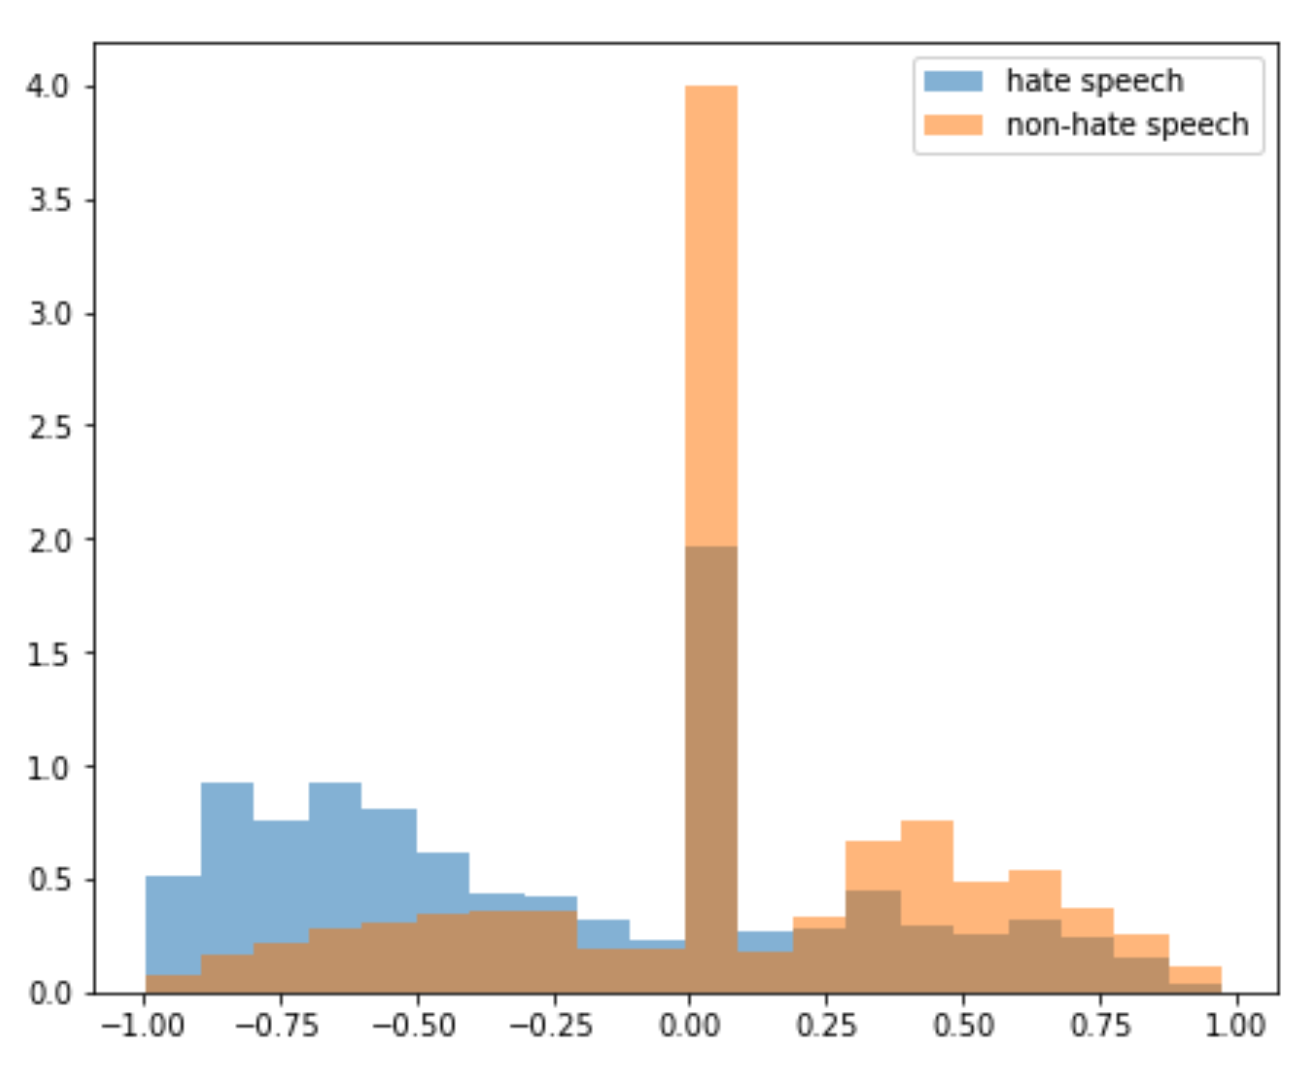
\includegraphics[width=0.7\linewidth]{figures/statistics_sentiment.png}
	\caption{Normalized distribution of sentiment score for hate speech vs. non-hate speech}
	\label{fig:statistics_sentiment}
\end{figure}

Further meaningful features were found using a dictionary approach by using the training data to generate a dictionary for hate speech and neutral words. The number of hateful words is distributed such that hate speech posts contain significantly more, whereas the number of neutral words does not differ much.
Examples for the most common hateful words found in hate speech posts are \enquote{fag}, \enquote{bitch}, \enquote{ass} or \enquote{nigga}. These words basically did not occur in non-hate speech posts. The most common neutral words are less informative, as the suffixes \enquote{ll} and \enquote{ve} are the most common ones for hate speech and non-hate speech posts.

\vspace{0.5cm}

Furthermore, we had an extensive look at unigrams, bigrams and trigrams for hate speech and these are significantly overrepresented in hate speech posts compared to non-hate speech posts. This especially holds true for the unigrams such as \enquote{white} which appears in 15\% of hate speech posts or \enquote{not} appearing in 9\% of hate speech posts. Both of these appear only half as often in non-hate speech posts.
The identified bigrams only show up in a very small percentage of posts, but significantly less in non-hate speech posts. Most common bigrams for hate speech are \enquote{white trash}, \enquote{look like} and \enquote{ass nigga}.

\vspace{0.5cm}

Lastly, the feature pattern-count can somewhat indicate hate speech, as the mean amount is higher for hate speech compared to non-hate speech. As one can see in \autoref{fig:statistics_pattern_count} hate speech tends to contain more patterns (which of course were trained by using the hate speech data).

\begin{figure}[ht]
	\centering
	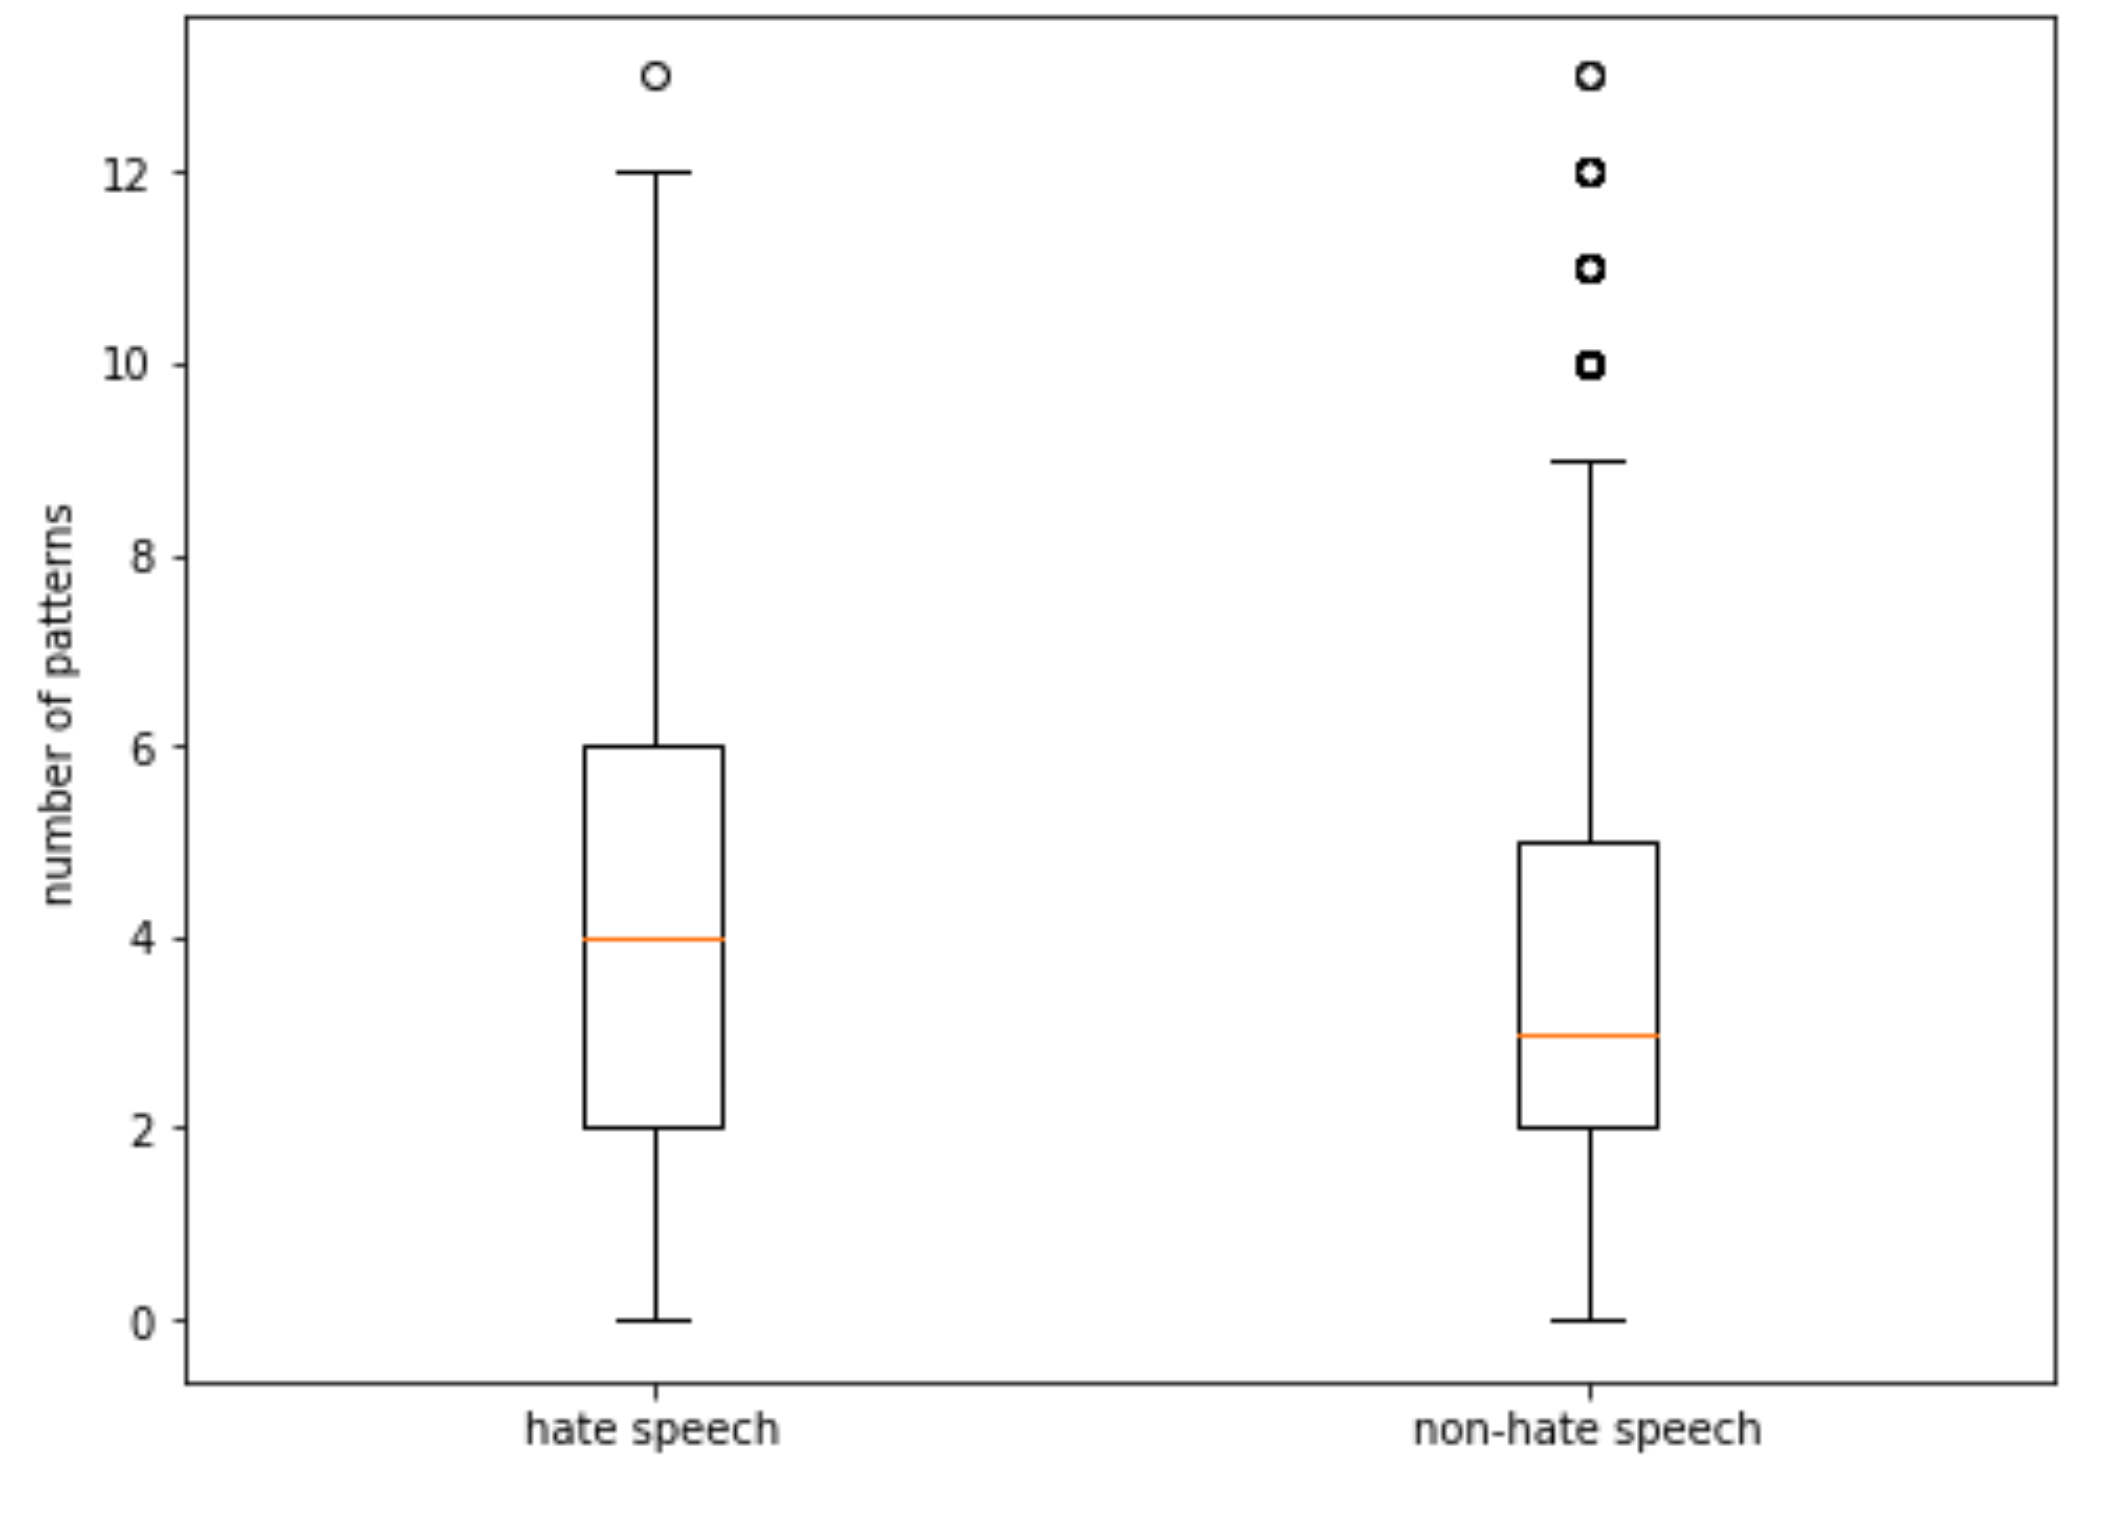
\includegraphics[width=0.7\linewidth]{figures/statistics_pattern_count.png}
	\caption{Boxplots comparing the number of patterns occurring in hate speech vs. non-hate speech}
	\label{fig:statistics_pattern_count}
\end{figure}

But maybe it would be worthwhile to have a closer look at the patterns and adjust them for some future work: when we look at single patterns, some occur more often in hate speech and some more often in non-hate speech (in our dataset). For example the pattern \enquote{adjective, noun (JJ, NN)} occurs in 56\% of hate speech and in 48\% of non-hate speech, whereas the pattern \enquote{determiner, noun} occurs in 5\% less hate speech posts than non-hate speech posts. So a more thorough analysis of these patterns could benefit this feature a lot, maybe by using individual features for each pattern. For example the biggest difference in occurrences is achieved by the pattern \enquote{personal pronoun, non-3rd person singular present verb (PRP, VBP)} with a 10\% difference.

\subsection{Comparison of the classifier results}
\label{ch:experimentDc}

Table \ref{Tab:unchanged} shows the performance metrics of the classifiers for the unbalanced dataset. 

\begin{table}[hbt!]
	\caption{Classifier results for unbalanced dataset}
	\label{Tab:unchanged}
	\begin{tabular}{|p{0.3\textwidth}|p{0.13\textwidth}|p{0.13\textwidth}|p{0.13\textwidth}|p{0.13\textwidth}|}
		\hline
		\textbf{classifier} & \textbf{precision} & \textbf{recall} & \textbf{accuracy} & \textbf{F1} \\ \hline
		Decision Tree       & \gradient{0.8756} & \gradient{0.9821} & \gradient{0.8671} & \gradient{0.9258} \\ \hline
		Random Forest       & \gradient{0.8809} & \gradient{0.9894} & \gradient{0.8782} & \gradient{0.9320} \\ \hline
		SVM                 & \gradient{0.8697} & \gradient{0.9927} & \gradient{0.8684} & \gradient{0.9272} \\ \hline
		Logistic Regression & \gradient{0.8831} & \gradient{0.9832} & \gradient{0.8760} & \gradient{0.9305} \\ \hline
		LSTM                & \gradient{0.9219} & \gradient{0.9567} & \gradient{0.8950} & \gradient{0.9390} \\ \hline
	\end{tabular}
\end{table}

All classifiers perform about equally well. And the achieved results are good with about 93\% for the F1-score. In the unbalanced case the conventional machine learning methods can definitely keep up with the neural network baseline. 

\subsection{Oversampled and undersampled datasets}
\label{ch:experimentDd}

Table \ref{Tab:undersampled} shows the performance metrics of the classifiers for the undersampled dataset and table \ref{Tab:oversampled} for the oversampled dataset. 

\begin{table}[hbt!]
	\caption{Classifier results for undersampled dataset}
	\label{Tab:undersampled}
	\begin{tabular}{|p{0.3\textwidth}|p{0.13\textwidth}|p{0.13\textwidth}|p{0.13\textwidth}|p{0.13\textwidth}|}
		\hline
		\textbf{classifier} & \textbf{precision} & \textbf{recall} & \textbf{accuracy} & \textbf{F1} \\ \hline
		Decision Tree       & \gradient{0.7202} & \gradient{0.7710} & \gradient{0.7431} & \gradient{0.7448} \\ \hline
		Random Forest       & \gradient{0.7261} & \gradient{0.8043} & \gradient{0.7573} & \gradient{0.7632} \\ \hline
		SVM                 & \gradient{0.7193} & \gradient{0.8375} & \gradient{0.7621} & \gradient{0.7739} \\ \hline
		Logistic Regression & \gradient{0.7246} & \gradient{0.8238} & \gradient{0.7621} & \gradient{0.7710} \\ \hline
		LSTM                & \gradient{0.9219} & \gradient{0.9567} & \gradient{0.8950} & \gradient{0.9390} \\ \hline
	\end{tabular}
\end{table}

\begin{table}[hbt!]
	\caption{Classifier results for oversampled dataset}
	\label{Tab:oversampled}
	\begin{tabular}{|p{0.3\textwidth}|p{0.13\textwidth}|p{0.13\textwidth}|p{0.13\textwidth}|p{0.13\textwidth}|}
		\hline
		\textbf{classifier} & \textbf{precision} & \textbf{recall} & \textbf{accuracy} & \textbf{F1} \\ \hline
		Decision Tree       & \gradient{0.7973} & \gradient{0.7919} & \gradient{0.7924} & \gradient{0.7946} \\ \hline
		Random Forest       & \gradient{0.8844} & \gradient{0.8557} & \gradient{0.8701} & \gradient{0.8698} \\ \hline
		SVM                 & \gradient{0.7648} & \gradient{0.8081} & \gradient{0.7767} & \gradient{0.7859} \\ \hline
		Logistic Regression & \gradient{0.7573} & \gradient{0.8081} & \gradient{0.7713} & \gradient{0.7819} \\ \hline
		LSTM                & \multicolumn{4}{|c|}{not measured} \\ \hline
	\end{tabular}
\end{table}

In the undersampled case all conventional machine learning methods perform about equally well. Compared to the results from unbalanced dataset the conventional classifiers perform worse. In contrast the neural network baseline can keep up with the results from the unbalanced case. So in this undersampled case the conventional machine learning methods cannot keep up with the neural network baseline.

In the oversampled case the results are located between the undersampled and the unbalanced case. An outstanding result is the Random Forest, which performs better then the other conventional machine learning methods. As already mentioned SMOTE is not able to generate new textual features for generating an oversampled dataset for the neural network baseline. That is why these results could not be measured.
